%%%% Paramétrage du cours %%%%
\def\xxactivite{Cours}

\def\xxauteur{Xavier Pessoles}
\fichefalse \proftrue \tdfalse \courstrue

\def\xxnumchapitre{Chapitre 5 \vspace{.2cm}}
\def\xxchapitre{\hspace{.12cm} Algorithmes dichotomiques et algorithmes gloutons}

\def\xxcompetences{%
\textsl{%
\textbf{Savoirs et compétences :}\\
\begin{itemize}[label=\ding{112},font=\color{bleuxp}] 
\item Algorithmes dichotomiques.
\end{itemize}
}}

\def\xxfigures{
%
\includegraphics[width=\linewidth]{fractale}
%\\
%\textit{Modèle du pilote hydraulique avec pilotage interactif.}
}%figues de la page de garde

\input{\repRel/Style/pagegarde_cours_minitoc}
\setlength{\columnseprule}{.1pt}

\vspace{2cm}
\pagestyle{fancy}
\thispagestyle{plain}

%%%%%%%%%%%%%%%%%%%%%%%


\section{Algorithmes dichotomiques}
\subsection{Introduction}
Les méthodes de résolutions par un algorithme dichotomique font partie des algorithmes basés sur le principe de " diviser pour régner ".\\
Elles utilisent la définition du terme \texttt{dichotomie} qui signifie diviser un tout en deux parties "opposées".\\
Certains algorithmes de tris sont basés sur ce principe de diviser pour régner.



Ce cours vous présente deux algorithmes dichotomiques :
\begin{itemize}
\item la recherche d'un élément dans une liste triée ;
\item la détermination de la racine d'une fonction quand elle existe.
\end{itemize}

\subsection{Recherche dichotomique dans une liste     {triée}: Principe}

Lorsque vous cherchez le mot <<~hippocampe~>> dans le dictionnaire, vous ne vous amusez pas à parcourir chaque page depuis la lettre a jusqu'à tomber sur le mot <<~hippocampe~>>...\\
Dans une liste triée, il y a plus efficace ! Par exemple dans le dictionnaire, vous ouvrez à peu près au milieu, et suivant si le mot trouvé est \og inférieur \fg \ ou \og supérieur \fg \ à <<~hippocampe~>> (pour l'ordre alphabétique), vous poursuivez votre recherche dans l'une ou l'autre moitié du dictionnaire.


\begin{prop}
On se donne une liste \texttt{L} de nombres de longueur \texttt{n},     {triée dans l'ordre croissant}, et un nombre \texttt{x0}. 

Pour chercher \texttt{x0}, on va couper la liste en deux moitiés et chercher dans la moitié intéressante et ainsi de suite.

On appelle \texttt{g}     {l'indice} de l'élément du début de la sous-liste dans laquelle on travaille et \texttt{d}     {l'indice} de l'élément de fin.

Au début, \texttt{g =0} et \texttt{d = n - 1} 

On souhaite construire un algorithme admettant l'invariant suivant:
\bigskip

\centerline{\fbox{si \texttt{x0} est dans \texttt{L} alors \texttt{x0} est dans la sous-liste \texttt{L[g:d]} (\texttt{g} inclus et \texttt{d} exclu).}}
\end{prop}



On va utiliser la méthode suivante :
\begin{itemize}
\item On compare \texttt{x0} à "l'élément du milieu" : c'est \texttt{L[m]} où \texttt{m = (g + d) // 2}
son indice est \texttt{m} =\texttt{ n//2} (division euclidienne)
$$\begin{array}{|c|c|c|c|c|c|c|c|c|} 
\hline \hspace*{3mm} & \hspace*{3mm} & \hspace*{3mm} &  \hspace*{3mm} & \hspace*{3mm} & \hspace*{3mm} & \hspace*{3mm} & \hspace*{3mm} & \hspace*{3mm}\\ \hline
\end{array}$$
\medskip
$$\begin{array}{|c|c|c|c|} 
\hline \hspace*{3mm} & \hspace*{3mm} & \hspace*{3mm} &  \hspace*{3mm} \\ \hline
\end{array}$$

\item Si \texttt{x0 = L[m]}, on a trouvé \texttt{x0}, on peut alors s'arrêter.
\item Si \texttt{x0} $<$ \texttt{L[m]}, c'est qu'il faut chercher dans la première moitié de la liste, entre \texttt{L[g]} et  \texttt{L[m-1]} (\texttt{L[m]} exclu).
%dans  {la première moitié de la liste \t{L[g:m]}}\\
\item Si \texttt{x0} $>$ \texttt{L[m]}, c'est qu'il faut chercher dans la seconde moitié de la liste, entre \texttt{L[m+1]} et \texttt{L[d]} (\texttt{L[m]} exclu).
\end{itemize}

On poursuit jusqu'à ce qu'on a trouvé \texttt{x0} ou lorsque l'on a épuisé la liste \texttt{L}.





\subsection{ Exemples d'application}
%\begin{enumerate}
%\item %En notant $g$ et $d$  les indices de gauche et de droite du morceau de la liste $l$ où l'on est en train de faire la %recherche, 
Indiquer pour les deux exemples suivants les valeurs successives de \texttt{g} et \texttt{d} :
\begin{enumerate}
\item \texttt{x0 = 5} et \texttt{L} $= \begin{array}{|c|c|c|c|c|c|c|c|c|} 
\hline -3 & 5 & 7 & 10 & 11 & 14 & 17 & 21 & 30 \\ \hline
\end{array}$


$\begin{cases}
g=0\\d=8\\m=4,L[m]>x0
\end{cases}
\begin{cases}
g=0\\d=3\\m=1,L[m]=x0
\end{cases}$.\\
C'est fini, on a bien trouvé $x_0$ dans la liste.


\item \texttt{x0 = 11} et \texttt{L} $= \begin{array}{|c|c|c|c|c|c|c|c|c|} 
\hline -2 & 1 & 2 & 7 & 8 & 10 & 13 & 16 & 17  \\ \hline
\end{array}$


$\begin{cases}
g=0\\d=8\\m=4,L[m]<x0
\end{cases},\begin{cases}
g=5\\d=8\\m=6,L[m]>x0
\end{cases}\begin{cases}
g=5\\d=5\\m=5,L[m]<x0
\end{cases}\begin{cases}
g=6\\d=5
\end{cases}$.

C'est fini, on a épuisé la liste \texttt{L} et on n'a pas trouvé $x0$.
\end{enumerate}


%\textbf{Remarque :} On en déduit que de manière générale, \texttt{m = (g + d) // 2} (division euclidienne)\\
 %- si \texttt{x0} $<$ \texttt{L[m]}, \texttt{g} est inchangé et \texttt{d} prend la valeur de \texttt{m}\\
 %- si \texttt{L[m]} $\leq$ \texttt{x0}, \texttt{d} est inchangé et \texttt{g} prend la valeur de \texttt{m}
 

\subsection{Implémentation en Python}


La fonction \texttt{recherche dichotomie} d'arguments une liste \texttt{L} et un élément \texttt{x0} renvoyant un booléen disant si \texttt{x0} est dans la liste \texttt{L} est proposée :



\begin{lstlisting}
def recherche dichotomie(L:list, x0:int)-> bool:
     n = len(L)
     g_ind = 0 # c'est l'indice de gauche
     d_ind = n - 1 # c'est l'indice de droite
     rep = False
     while g ind <= d_ind and rep == False:
         # si x0 est dans L alors L[g ind] <= x0 <= L[d ind]     {invariant}
         m = (d ind + g ind) // 2 
         if x0 == L[m]:
             rep = True
         elif x0 < L[m]:
             d_ind = m - 1
          else:
             g_ind = m + 1
           # si x0 est dans L alors L[g_ind] <= x0 <= L[d_ind]     {invariant}
     return(rep)
\end{lstlisting} 



%\begin{python}
%def dichotomie(L, x0):\\
%     n = len(L)\\
%     g = 0\\
%     d = n\\
%     while  {d - g > 1:}\\
%         m =  {(d + g) // 2} \\
%         if  {x0 < L[m]}\\
%              {d = m}\\
%          else:\\
%              {g = m}\\
%     return  {x0 == L[g]}
%\end{python}
\textbf{Remarque :} La terminaison de l'algorithme est obtenue avec $d-g$ qui est un entier positif qui décro\^{i}t strictement à chaque passage dans la boucle \texttt{while} et joue le rôle de variant.
%\end{enumerate}


\subsection{Détermination de la racine d'une fonction par dichotomie}

\subsubsection{Principe théorique de la méthode par dichotomie}
On considère une fonction $f$ vérifiant : 
\begin{center} $f$ continue sur $\verb![!a,b\verb!]!$ ;  $f(a)$ et $f(b)$ de signes opposés.
\end{center} Le théorème des valeurs intermédiaires nous assure que $f$ possède au moins un zéro $\ell$ entre $a$ et $b$. La preuve, vue en cours de mathématiques, repose sur la méthode de dichotomie. Prenons le cas $f(a)<0$ et $f(b)>0$ et posons $g_0=a$, $d_0=b$. 
%\begin{center}
%\begin{tikzpicture}%[scale=2,xmin=-2.5,xmax=2.5,ymin=-1.5,ymax=1.5]
%\shorthandoff{:};
%%\draw[->] (\xmin,0)--(\xmax,0);
%\draw[->] (-2.5,0)--(2.5,0);
%%\draw[->] (-2.25,\ymin)--(-2.25,\ymax);
%\draw[->] (-2.25,-1.5)--(-2.25,1.5);
%\fenetre
%\draw[domain=-2:2, samples=200, very thick]  plot ({\x},{((\x)^5+3*(\x)-7)/34});
%\draw (-2,0)node{$\cdot$};
%\draw (-1,0)node{$\cdot$};
%\draw (1,0)node{$\cdot$};
%\draw (0,0)node{$\cdot$};
%\draw (2,0)node{$\cdot$};
%\draw (-2 , 0) node[below] {$a$};
%\draw (2 , 0) node[below] {$b$};
%\draw (1.26 , 0) node[below] {$\ell$};
% \end{tikzpicture}
% \end{center}
 On considère $m_0 = \dfrac{g_0+d_0}{2}$ et on évalue $f(m_0)$ : 
\begin{itemize}
 \item Si $f(m_0)\geq 0$, on va poursuivre la recherche d'un zéro dans l'intervalle  {$[g_0,m_0]$} \\On pose donc  : 
 $g_1 =  {g_0} \quad ;\quad  d_1 =  {m_0}$\vspace*{2mm}
  \item Sinon,  la recherche doit se poursuivre  dans l'intervalle  {$[m_0,d_0]$} \\ On pose donc  : 
 $g_1 =  {m_0} \quad ; \quad d_1 =  {d_0}$\vspace*{2mm}
 \item On recommence alors en considérant $m_1 = \dfrac{g_1+d_1}{2}$...\\
 \end{itemize}


 \begin{enumerate}
 \item Par quoi peut-on remplacer la condition "$f(m_k)\geq 0$" dans le cas général où $f(a)$ et $f(b)$ sont de signes contraires (pas forcément $f(a)<0$ et $f(b)>0$) ?

 \item \`A quelle condition sur $g_n$ et $d_n$ s'arrête-t-on, si l'on souhaite que $g_n$ et $d_n$ soient des solutions approchées de $\ell$ à une précision $\varepsilon$ ?

 \item  Au lieu de renvoyer $g_n$ et/ou $d_n$ comme valeurs approchées de $\ell$, que pourrait-on prendre ? 
 
 Que mettre comme condition d'arrêt pour avoir une précision $\varepsilon$  ? 

 \item Un étudiant propose de tester si $f(m_k)=0$.  Qu'en pensez-vous ?

\end{enumerate}


\subsection{Implémentation en Python et avec scipy}
\'Ecrivons une fonction \texttt{zero dichotomie(f:function,a:float,b:float,epsilon:float)->float} d'arguments une fonction \texttt{f}, des flottants \texttt{a} et \texttt{b} (tels que \texttt{a < b}), et  la précision voulue \texttt{epsilon} (flottant strictement positif). Cette fonction renverra une valeur approchée à \texttt{epsilon} près d'un zéro de \texttt{f}, compris entre \texttt{a} et \texttt{b}, obtenue par la méthode de dichotomie.

\begin{lstlisting}
def zero dichotomie(f:function, a:float, b:float, epsilon:float):
     val g = a # c'est un flottant
     val d = b # c'est un flottant
     while val d - val g > 2 * epsilon :
          m = (val g + val d) / 2
          if f(val g) * f(m) <= 0:
               val d = m
          else:
               val g = m
     return ((val g + val d) / 2)
\end{lstlisting}

Effectuons un test avec la fonction $f : x \mapsto x^2-2$ sur l'intervalle $\verb![!1,2\verb!]!$, avec une précision de $10^{-6}$ :
 
\begin{lstlisting}
def f(x):
     return(x ** 2 - 2)
print (zero dichotomie(f, 1, 2, 10**(-6)))

# il s'affichera : 1.4142141342163086
\end{lstlisting}
%\begin{algorithm}
%\begin{algorithmic}
%
% {
%\STATE $g \leftarrow a$
%\STATE $d \leftarrow b$
%\WHILE{$d-g> 2\varepsilon$}
%\STATE $m \leftarrow (g+d)/2$
%\IF{$f(g)f(m)\leq 0$}
%\STATE $d \leftarrow m$
%\ELSE
%\STATE $g \leftarrow m$
%\ENDIF
%\ENDWHILE
%\STATE renvoyer $\dfrac{g+d}{2}$}
%~\newline
%~\newline
%~\newline
%\end{algorithmic}
%\end{algorithm}
% 

%\subsection{Fonction prédéfinie dans scipy}
Une telle fonction est déjà prédéfinie dans la bibliothèque \texttt{scipy.optimize}, la fonction \texttt{bisect} \linebreak (la méthode de dichotomie s'appelle aussi la méthode de la \textit{bisection}) : 
\begin{lstlisting}
import scipy.optimize as spo\\[2mm]
print (spo.bisect(f, 1, 2)) \\
# il s'affichera : 1.4142135623724243
\end{lstlisting}
La précision est un argument optionnel (à mettre après \texttt{f}, \texttt{a} et \texttt{b}) et vaut $10^{-12}$ par défaut.



\section{Présentation des algorithmes Gloutons}

\textit{
En informatique, un algorithme glouton (greedy algorithm en anglais, parfois appelé aussi algorithme gourmand) est un algorithme qui suit le principe de faire, étape par étape, un choix optimum local. Dans certains cas, cette approche permet d'arriver à un optimum global, mais dans le cas général c'est une heuristique \footnote{une heuristique est une méthode de calcul qui fournit rapidement une solution réalisable, pas nécessairement optimale ou exacte, pour un problème d'optimisation difficile.}} (Wikipédia).\\

Les algorithmes gloutons sont utilisés dans des problèmes d’optimisation. Un problème d’optimisation consiste à déterminer les valeurs des paramètres permettant de :
\begin{itemize}
	\item minimiser ou maximiser une fonction objectif ;
	\item satisfaire une ou des fonctions contraintes (il existe des problèmes avec ou sans contrainte).
\end{itemize}

\subsection{Choix d'itinéraire}
 
On peut citer par exemple le problème du choix d’itinéraire dans un réseau routier : il faut déterminer le trajet de sorte à minimiser le temps de parcours, tout en respectant un ensemble de contraintes : circuler sur les routes (on ne coupe pas à travers champs !) et respecter les sens de circulation.

\subsection{Recherche d'un minimum d'une fonction} 
Voici un second exemple : 
\begin{itemize}
	\item 	La recherche du minimum de la fonction $f:x \longmapsto x^2-x-2$ est un problème d’optimisation sans contrainte.
	\item		La recherche du minimum de la fonction $f:x \longmapsto x^2-x-2$ sous la contrainte $x^3\geq8$ est un problème d’optimisation sous contrainte (contrainte d’inégalité). L’optimum est alors $x=2$ et $f(2)=0$. L’ensemble des solutions vérifiant les contraintes sont appelées solutions valides ou valables.
\end{itemize}


\begin{minipage}{.6\textwidth}
On distingue également plusieurs types d’optimum :
\begin{itemize}
	\item optimum global ;
	\item	optimum local strict (unique dans un intervalle réduit);
	\item	optimum local (non unique dans un intervalle réduit).
\end{itemize}
\end{minipage}
\hfill
\begin{minipage}{.35\textwidth}
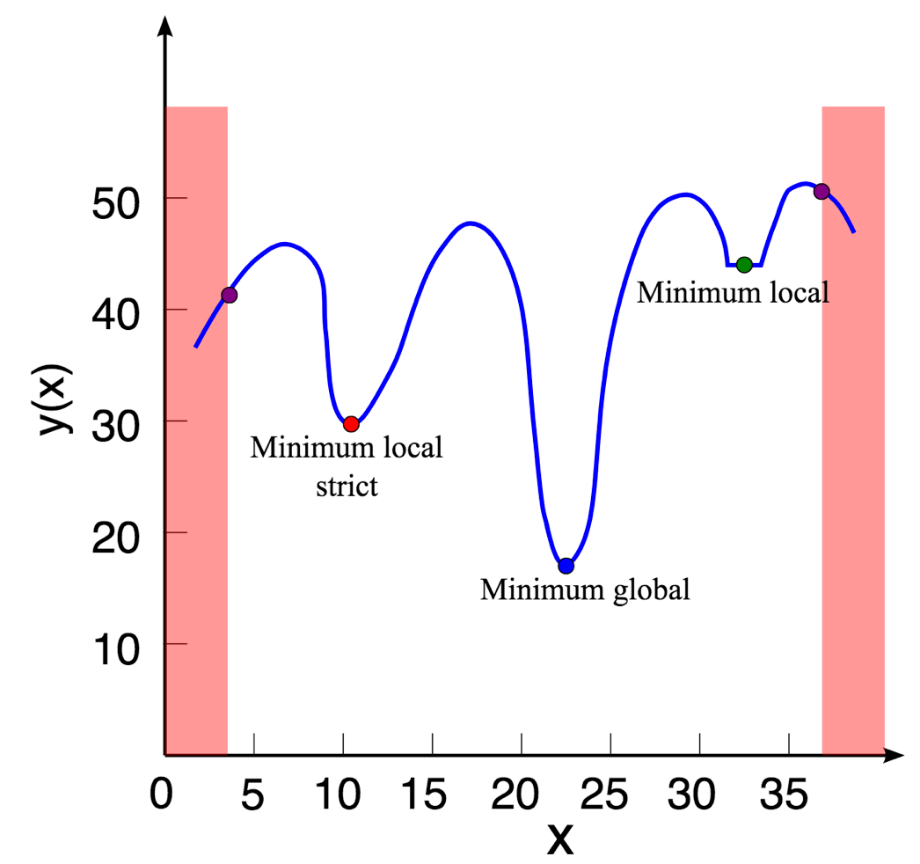
\includegraphics[scale=0.5]{optimums.png}
\end{minipage}

La méthode gloutonne est très puissante et fonctionne bien pour toutes sortes de problèmes. L'algorithme de \texttt{Dijkstra}, que l'on étudiera en fin d'année, qui calcule des plus courts chemins à origine unique, peut être vu comme une application de la méthode gloutonne.

\subsection{\'Eléments de la stratégie gloutonne}

Le processus pour mettre au point un algorithme glouton présente plusieurs étapes :

\begin{enumerate}
\item Détermination de la sous-structure optimale du problème ;
\item Développement d'une solution formulée par récurrence ;
\item Démonstration que, si nous avons fait un choix glouton, il ne reste qu'un seul sous-problème ;
\item Démonstration qu'il est toujours sûr de faire le choix glouton. (Les étapes 3 et 4 peuvent se faire dans n'importe quel ordre.)
\item \'Ecriture d'un algorithme récursif ou itératif.
\end{enumerate}

\subsubsection{Propriété de choix glouton}

La première caractéristique principale est la propriété de choix glouton : on peut assembler une solution globalement optimale en effectuant des choix localement optimaux (gloutons). Autrement dit, quand on considère le choix à faire, on fait le choix qui paraît le meilleur pour le problème courant, sans tenir compte des résultats des sous-problèmes.


\subsubsection{Exemple : un problème d'organisation}

\textit{source : algorithmes gloutons - eduscol}

Des conférenciers sont invités à présenter leurs exposés dans une salle. Mais leurs disponibilités ne leur permettent d'intervenir qu'à des horaires bien définis. Le problème est de construire un planning d'occupation de la salle avec le plus grand nombre de conférenciers.\\
Désignons par $n$, entier naturel non nul, le nombre de conférenciers. Chacun d'eux, identifié par une lettre $C_i$, où $i$ est un entier compris entre 0 et $n-1$, est associé à un intervalle temporel \verb![!di, fi\verb![! où di et fi désignent respectivement l'heure de début et l'heure de fin de l'intervention. Afin de dégager une tactique de résolution du problème, commençons par analyser plusieurs situations.

\subsubsection{Les créneaux ne se chevauchent pas}

Une telle situation est simple puisque tous les conférenciers peuvent intervenir sur des créneaux horaires disjoints.

\subsubsection{Les créneaux se chevauchent}

Dans cette situation, les intervalles ne sont plus disjoints. Nous dirons que ces intervalles ne sont pas compatibles. Des choix doivent être faits et certains conférenciers peuvent ne pas être retenus pour construire un planning.



%\newpage
%\renewcommand{\contentsname}{Plan du cours}
%\tableofcontents




